\documentclass[10pt]{article}

\usepackage[utf8x]{inputenc}
\usepackage[english,italian]{babel}
\usepackage{graphicx} 
\usepackage{booktabs}
\usepackage{caption}
\usepackage{textgreek}
\usepackage{tabularx}
\usepackage{amsmath,amssymb,stackengine}
\usepackage{authblk}
\usepackage{xcolor}


\usepackage{geometry} % to change the page dimensions
\geometry{a4paper} % or letterpaper (US) or a5paper or....
% \geometry{margin=2in} % for example, change the margins to 2 inches all round
% \geometry{landscape} % set up the page for landscape
%   read geometry.pdf for detailed page layout information

\usepackage{graphicx} % support the \includegraphics command and options

% \usepackage[parfill]{parskip} % Activate to begin paragraphs with an empty line rather than an indent

%%% PACKAGES
\usepackage{booktabs} % for much better looking tables
\usepackage{array} % for better arrays (eg matrices) in maths
\usepackage{paralist} % very flexible & customisable lists (eg. enumerate/itemize, etc.)
\usepackage{verbatim} % adds environment for commenting out blocks of text & for better verbatim
\usepackage{subfig} % make it possible to include more than one captioned figure/table in a single float
% These packages are all incorporated in the memoir class to one degree or another...

%%% HEADERS & FOOTERS
\usepackage{fancyhdr} % This should be set AFTER setting up the page geometry
\pagestyle{fancy} % options: empty , plain , fancy
\renewcommand{\headrulewidth}{0pt} % customise the layout...
\lhead{}\chead{}\rhead{}
\lfoot{}\cfoot{\thepage}\rfoot{}

\usepackage{sectsty}
\allsectionsfont{\sffamily\mdseries\upshape} 

\usepackage[nottoc,notlof,notlot]{tocbibind}
\usepackage[titles,subfigure]{tocloft} 

\renewcommand{\cftsecfont}{\rmfamily\mdseries\upshape}
\renewcommand{\cftsecpagefont}{\rmfamily\mdseries\upshape} 
\newcommand*{\hham}{\mathcal{H}}
\newcommand*{\xx}{\vec{x}}
\newcommand*{\kk}{\vec{k}}
\newcommand*{\qq}{\vec{q}}
\newcommand*{\p}{\varphi}
\newcommand*{\zpart}{\mathcal{Z}}
\newcommand*{\w}{\Bigl}
\newcommand*{\lapint}{\int_{a-i\infty}^{a+i\infty}\frac{dz}{2\pi i}}

\definecolor{carmine}{rgb}{0.59, 0.0, 0.09}


\selectlanguage{english}

\title{{\bf Notes on ecosystems stability}}

\author{Onofrio Mazzarisi}

%\affil{{\it Max Planck Institute for Mathematics in the Sciences, Leipzig, Germany}}

\begin{document}

\selectlanguage{english}

%\begin{abstract}
%\end{abstract}

\maketitle

\section{Super quadratic self-regulation}
Consider the case as in the draft but with production 
\begin{equation}
    P(n_i) = rn_i - rn_i^l/K^l \qquad \textrm{(super-regulated)} \, ,
\end{equation}
with $l\geq 2$, recovering the logistic case for $l=2$.
Following the same notation and calculation as in the draft we have,
in this case, the following community matrix
\begin{equation}
   C =  -DA -\frac{(l-1)r}{K^l}D^{l-1} \, .
\end{equation}
In this case we have that instabilities sets in if
\begin{equation}
    \sum_i \frac{1}{|\mu -(l-1)r(n_i^*)^{l-2}/K^l|^2}\geq 1/\sigma^2 \, ,
\end{equation}
which correctly recover the logistic case for $l=2$.
The stability condition for $l>2$ can be approximated by
\begin{equation}
    \sigma \leq (l-1)\sqrt{S}\mu r/K^l \, ,
\end{equation}
where we used the fact that
\begin{equation}
    (n_i^*)^{l-2} = \sum_j A_{ij}n_j^*/n_i^* - r/n_i^* = \mathcal{O}(\mu S) \, .
\end{equation}

\section{General}

Consider the production function
\begin{equation}
    P(n_i) = r\left(n_i^k - n_i^l/K^{l-k}\right) \qquad \textrm{(general)} \, ,
\end{equation}
with $k\leq1$, $l\geq2$ and the carrying capacity $K$ either finite or infinite.
We recover the logistic case for $k=1$ and $l=2$, the sublinear
case for $l=2$ and $K\to\infty$ and the super-regulated case for $k=1$.
The community matrix reads
\begin{equation}
    C =  -DA -(1-k)rD^{k-1} -\frac{(l-1)r}{K^{l-k}}D^{l-1} \, ,
\end{equation}
therefore the system becomes unstable if 
\begin{equation}
    \sum_i \frac{1}{|\mu -(1-k)r(n_i^*)^{k-2} -(l-1)r(n_i^*)^{l-2}/K^{l-k}|^2}\geq 1/\sigma^2 \, .
\end{equation}
It seems less straightforward to find an approximate
stability condition in terms of $S$ in this case.
The fact that we have
\begin{equation}
    r(n_i^*)^{k-2} - r(n_i^*)^{l-2}/K^{l-k} = \sum_j A_{ij}n_j^*/n_i^* = \mathcal{O}(\mu S) \, ,
\end{equation}
could be maybe used but the terms appear with weights in the equaition for stability.
I will explore further.

\section{More general}
Consider the system of $S$ species
\begin{equation}
    \frac{dn_i}{dt} = P(n_i) - n_i\sum_{j\neq i}A_{ij}n_j \, ,
\end{equation}
where the summation runs over all the species and we leave the production function generic
and $A$ is a matrix with zero diagonal and off-diagonal elements gaussianly
ditrubuted with mean $\mu$ and standard deviation $\sigma$.
The community matrix reads in this case
\begin{equation}
    C = -D(n^*)A - D(P(n^*)/n^*-P'(n^*)) \, ,
\end{equation}
where the notation $D(x)$ stands for a diagonal matrix filled 
with the components of the vector
$x$ and $P(n^*)=(P(n_1^*), ..., P(n_S^*))$ and $P'(n^*)=(dP(n_1^*)/dn_1^*, ..., dP(n_S^*)/dn_S^*)$.

We have instability when
\begin{equation}
    \sum_i \frac{1}{|\mu -P(n_i^*)/(n_i^*)^2+P'(n_i^*)/n_i^*|^2}\geq 1/\sigma^2 \, .
\end{equation}

\section{Sublinear production across a gradient}
Dynamical sublinear production does not generally leads to 
sublinear production across a biomass gradient.
Nonetheless I argue here that, although not sufficient, it might be necessary for (or at least
functional to) sublinear scaling across a biomass gradient.
Therefore it may nicely fit with the findings that dynamical sublinear
scaling leads to incresing stability for increasing richness.

\subsection{Single population}
Let me focus on a single population example to calrify the ideas.
Consider a production function of the form
\begin{equation}
    P(n) = r n^k \, ,
\label{eq: production}
\end{equation}
where $n$ is the biomass density of the population, $k\leq1$
specify the intensity of sublinear dynamical scaling (linear when $k=1$) 
and $r$ is the parameter that allows to move across a biomass gradient.
Consider then a self-regulation term of the form
\begin{equation}
    Q(n) = s n^l \, .
\end{equation} 
The evolution equaiton for the population is 
\begin{equation}
    \frac{dn}{dt} = P(n) - Q(n) = r n^k - s n^l \, ,
\end{equation} 
which reduces to logistic growth for $k=1$ and $l=2$.
The equilibrium is given by
\begin{equation}
    n^* = \left(\frac{r}{s}\right)^{1/(l-k)} \, ,
\label{eq: equilibrium single}
\end{equation}
and the stability condition is given by
\begin{equation}
    \frac{d\left[P(n)-Q(n)\right]}{dn}\bigg|_{n=n^*} < 0 \, ,
\end{equation}
which leads, after some calculations, to the condition
\begin{equation}
    k<l \, ,
\end{equation}
independent from $r$ and $s$.

It possible to appreciate from Eq.~(\ref{eq: equilibrium single})
that $k>l$, apart from making the equilibrium unstable, implies that
the stationary population \textit{decreases} for increasing $r$,
which is biologically unreasonable.

The equilibrium production scales, at varying growth rate $r$,
as $P(n^*)=s(n^*)^l$ as can be noted by Eq.~(\ref{eq: equilibrium single})
for $r$ and then substituting it in the defining Eq.~(\ref{eq: production})
or simply by considering the dynamical equation at stationarity.
Notice that, if $s$ is varied instead, the exponent
of dynamical and across-biomass-gradient production coincide, 
consistently with what is proposed in the 2015 paper.
I discuss anyway why $r$ is preferable to be changed instead of $s$ elsewhere.
Figure~\ref{fig. example} shows an example with specific parameters.

\begin{figure}[h!]
    \centering
    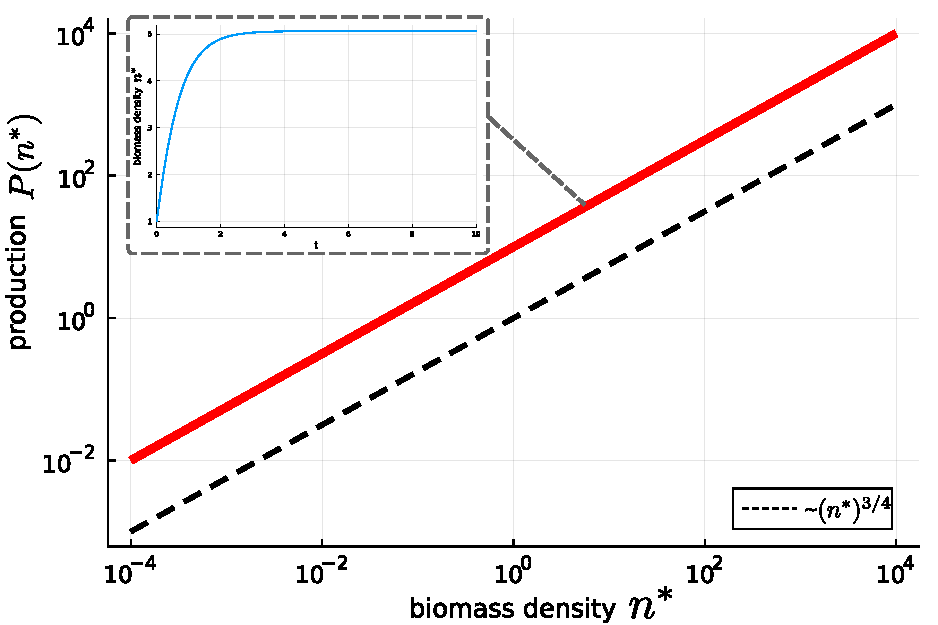
\includegraphics[width=.8\textwidth]{fig/single-pop.pdf}
    \caption{Production versus biomass density for $r\in[1,100]$,
    $s=10$, $k=1/2$ and $l=3/4$. In the inset the equilibration process
    for $r=10$.}
    \label{fig. example}
\end{figure}

In summary, the production across a biomass gradient 
scales as $(n^*)^l$ but in order for this to be biologically meaningful
and for the stationary solution to be stable an exponent $k<l$
for the dynamical produciton is needed.
In order to have sublinear $P(n^*)$ across a biomass gradient
we need therefore $k<l<1$.

\subsection{Large ecosystem}
Consider a complex large ecosystem 
described by the set of equations
\begin{equation}
\frac{dn_i}{dt} = r_in_i^k - Q(\vec{n}) \, .   
\end{equation}
For the species $i$ to exhibits
sublinear produciton scaling across a biomass gradient
one should have $Q(\vec{n})\sim n_i^l$, with $k<l<1$.


\newpage

\bibliography{Bib/library.bib}

\bibliographystyle{unsrt}

\end{document}